% RF coupling
\chapter{RF Coupling}
\label{chap:rf_coupling}
\margintoc

\section{Waves In Plasma}
\subsection{Cold Plasma Waves}
\subsection{Dispersion Relation}
\chapter{Dispersion Relation}
\section{Vacuum Dispersion Relation}
In a non-dispersive isotropic homogeneous non-lossy dielectric medium, such as vacuum (or air), the wavevector $\mathbf{k}=k\mathbf{\hat{k}}$ direction is given by:
\begin{equation}
\mathbf{\hat{k}}\cdot\mathbf{E}=0
\;\;\;\;\;\;
\mathbf{H}=\frac{n}{Z_{0}}\hat{\mathbf{k}}\times\mathbf{E}\label{eq:vecteur_onde_vide}
\end{equation}
where $\mathbf{\hat{k}}$ the unit vector in the direction of $\mathbf{k}$, $k=|\mathbf{k}|=n k_{0}$ is the wavenumber and $n=\sqrt{\varepsilon_{r}}$ the medium optical index. $Z_{0}=\sqrt{\frac{\mu_{0}}{\varepsilon_{0}}}=\mu_{0}c_{0}=\frac{1}{\varepsilon_{0}c_{0}}$ is the \emph{vacuum impedance}. The wave equation in such a medium is:
\begin{equation}
\mathbf{k} \times \mathbf{k} \times \mathbf{E} + k^{2} \mathbf{E} = \mathbf{0}
\end{equation}

The condition for that system of 3 equations and 3 unknowns $(E_{x},E_{y},E_{z})$ to have a non-trivial solution, consists in solving the \emph{dispersion relation} between the wavevector $\mathbf{k}$ and the angular frequency $\omega$, i.e. $\mathbf{k}(\omega)$. In this medium, this relation is simple (TODO demo): $k=\sqrt{\mu\varepsilon}\omega=\frac{c}{n}\omega$((7.4) \sidecite{Jackson1998})\sidenote{While in a lossy medium $k^{2}=\mu\varepsilon\omega^{2}-j\omega\mu\sigma$ (sec. 8.2 \sidecite{Bladel2007}).}.

\subsection{Cold Plasma Dispersion Relation}
Starting from Maxwell equations expressed in the $k-\omega$ domain (\ref{eq:k-omegaMaxwellEquations}) and assuming that the dispersion relations are of the form (\ref{eq:k-omegaDispersionRelation}), with the supplementary assumption that the medium is non magnetic (i.e. $\boldsymbol{\mu}=\mu_0$), one has thus:
\begin{subequations}
	\begin{align}
		\mathbf{k} \times \boldsymbol{\mathcal{E}} (\mathbf{k}, \omega) 
		=& 
		\omega \mu_0 \boldsymbol{\mathcal{H}}(\mathbf{k}, \omega) 
		\\
		\mathbf{k} \times \boldsymbol{\mathcal{H}} (\mathbf{k}, \omega) 
		=& 
		\left(
		-\omega \boldsymbol{\varepsilon} (\mathbf{k}, \omega) 
		+ 	
		j\boldsymbol{\sigma} (\mathbf{k}, \omega) 
		\right) \cdot 
		\boldsymbol{\mathcal{E}}(\mathbf{k}, \omega)
		\\
		\mathbf{k}  \cdot \boldsymbol{\varepsilon}(\mathbf{k}, \omega)  \cdot \boldsymbol{\mathcal{E}} (\mathbf{k}, \omega) 
		=& jq_v(\mathbf{k}, \omega) 
		\\
		\mathbf{k}  \cdot \boldsymbol{\mathcal{H}} (\mathbf{k}, \omega) 
		=& 0	
	\end{align}
\end{subequations}
combining the first two equations leads to the propagation equation:
\begin{equation}
\mathbf{k} \times \mathbf{k} \times \boldsymbol{\mathcal{E}} (\mathbf{k}, \omega) 
-
\left(
-\omega^2 \mu_0 \boldsymbol{\varepsilon} (\mathbf{k}, \omega) 
+ 	
j\omega\mu_0\boldsymbol{\sigma} (\mathbf{k}, \omega) 
\right) \cdot 
\boldsymbol{\mathcal{E}}(\mathbf{k}, \omega)
=
\boldsymbol{0}
\end{equation}
Let's define the equivalent relative dielectric tensor $\mathbf{K}$ such as:
\begin{equation}
\mathbf{K}(\mathbf{k},\omega)
=
\frac{j}{\omega\varepsilon_0}\boldsymbol{\sigma} (\mathbf{k}, \omega)
-\mathbf{I}
\end{equation}
then,
\begin{equation}
\mathbf{k} \times \mathbf{k} \times \boldsymbol{\mathcal{E}} (\mathbf{k}, \omega) 
- k_0^2
\mathbf{K}(\mathbf{k}, \omega) \cdot 
\boldsymbol{\mathcal{E}}(\mathbf{k}, \omega)
=
\boldsymbol{0}
\end{equation}
where $k_0=\frac{\omega}{c}$
% Dans un plasma froid magnétisé, la situation est radicalement différente,
% car les courants de polarisation générés par les mouvements électroniques
% et ioniques modifient la polarisation des ondes planes ainsi que leur
% dispersion. Différentes branches de dispersion, ou \emph{modes}, apparaissent\cite[chap.8]{Rax2005}. 
% 
% On rappelle l'expression des équations de Maxwell en régime harmonique
% pour une onde plane de vecteur d'onde $\mathbf{k}$ :
% 
% \begin{eqnarray}
% \mathbf{k}\times\mathbf{E} & = & \omega\mu_{0}\mathbf{H}\\
% \mathbf{k}\times\mathbf{H} & = & -\omega\varepsilon_{0}\mathbf{K}\cdot\mathbf{E}
% \end{eqnarray}
% Pour déterminer les propriétés de ces modes, on étudie les solutions
% de l'\emph{équation d'onde} déduite des deux précédentes équations\footnote{NB : L'équation d'onde ne dépend pas de la convention temporelle choisie.}
% :
% 
% \begin{equation}
% \mathbf{n}\times\mathbf{n}\times\mathbf{\tilde{E}}+\mathbb{K}\cdot\mathbf{\tilde{E}}=\mathbf{0}\label{eq:Helmoltz}
% \end{equation}
% où $\mathbf{n}=\mathbf{k}/k_{0}$ correspond au vecteur d'indice de
% réfraction, dont la direction est celle du vecteur d'onde $\mathbf{k}$
% et l'amplitude celle de l'indice de réfraction. A priori, la matrice
% $\mathbb{K}$ dépend des trois composantes du vecteur d'onde $\mathbf{k}$.
% En choisissant le système de coordonnées cartésien l'équation \ref{eq:Helmoltz}
% peut s'écrire sous forme matricielle\footnote{On peut s'économiser un peu de calcul vectoriel grâce à un peu d'algèbre
% et le formalisme des dyadiques\cite{Belov2003,Lindell1995}. En utilisant
% l'identité ``BAC-CAB'', le double produit vectoriel s'écrit $\mathbf{n}\times\mathbf{n}\times\mathbf{\tilde{E}}=\mathbf{n}\left(\mathbf{n}\cdot\mathbf{\tilde{E}}\right)-\mathbf{\tilde{E}}\left(\mathbf{n}\cdot\mathbf{n}\right)=\mathbf{n}\left(\mathbf{n}\cdot\mathbf{\tilde{E}}\right)-n^{2}\mathbf{\tilde{E}}$.
% Avec l'opération dyadique $\mathbf{n}\left(\mathbf{n}\cdot\tilde{\mathbf{E}}\right)=\mathbf{nn}\cdot\mathbf{\tilde{E}}$
% et $\mathbb{I}=\mathbf{xx}+\mathbf{yy}=\mathbf{zz}$ l'opérateur dyadique
% unité vérifiant $\mathbf{\tilde{E}}=\mathbb{I}\cdot\tilde{\mathbf{E}}$on
% peut alors factoriser l'équation \ref{eq:Helmoltz} en un opérateur
% dyadique $\left(\mathbf{nn}-n^{2}\mathbb{I}+\mathbb{K}\right)\cdot\tilde{\mathbf{E}}=\mathbf{0}$
% qui donne directement l'expression matricielle de l'équation \ref{eq:relation_disp_matr}.} :
% \begin{equation}
% \left(\begin{array}{ccc}
% K_{xx}-n_{y}^{2}-n_{z}^{2} & K_{xy}+n_{x}n_{y} & K_{xz}+n_{x}n_{z}\\
% K_{yx}+n_{x}n_{y} & K_{yy}-n_{x}^{2}-n_{z}^{2} & K_{yz}+n_{y}n_{z}\\
% K_{zx}+n_{x}n_{z} & K_{zy}+n_{y}n_{z} & K_{zz}-n_{x}^{2}-n_{y}^{2}
% \end{array}\right)\left(\begin{array}{c}
% \tilde{E_{x}}\\
% \tilde{E}_{y}\\
% \tilde{E}_{z}
% \end{array}\right)=\mathbf{0}\label{eq:relation_disp_matr}
% \end{equation}
%  Si l'on suppose en plus que le vecteur d'onde $\mathbf{k}$ (ie.
% la propagation de l'onde) soit contenu dans le plan $x-z$ (ie $k_{y}=n_{y}=0$),
% l'équation précédente devient :
% 
% \begin{equation}
% \left(\begin{array}{ccc}
% K_{xx}-n_{z}^{2} & K_{xy} & K_{xz}+n_{x}n_{z}\\
% K_{yx} & K_{yy}-n_{x}^{2}-n_{z}^{2} & K_{yz}\\
% K_{zx}+n_{x}n_{z} & K_{zy} & K_{zz}-n_{x}^{2}
% \end{array}\right)\left(\begin{array}{c}
% \tilde{E_{x}}\\
% \tilde{E}_{y}\\
% \tilde{E}_{z}
% \end{array}\right)=\mathbf{0}\label{eq:relation_disp_matr_full}
% \end{equation}
% Si le plasma est homogène (indépendant de $\mathbf{r}$) on peut exploiter
% l'équivalence entre toutes les directions perpendiculaires au champ
% magnétique statique pour prédire que $\mathbb{K}$ doit être fonction
% de $k_{\parallel}$et $k_{\perp}^{2}$ seulement. 
% 
% \begin{figure}
% \begin{centering}
% \includegraphics[width=0.5\textwidth]{figures/geometrie_dispersion_plasma}
% \par\end{centering}
% \caption{Géométrie cartésienne du milieu plasma.\label{fig:G=0000E9om=0000E9trie-cart=0000E9sienne-plasma}}
% \end{figure}
% 
% Si $\mathbb{K}$ est le tenseur de permittivité d'un plasma froid
% (\ref{eq:tenseur_stix}) définit dans l'annexe \ref{sec:Tenseur-de-permittivit=0000E9},
% c'est-à-dire tel que $z$ soit parallèle au champ magnétique (Figure
% \ref{fig:G=0000E9om=0000E9trie-cart=0000E9sienne-plasma}), alors
% on a:
% 
% \begin{equation}
% \left(\begin{array}{ccc}
% S-n_{z}^{2} & jD & n_{x}n_{z}\\
% -jD & S-n_{x}^{2}-n_{z}^{2} & 0\\
% n_{x}n_{z} & 0 & P-n_{x}^{2}
% \end{array}\right)\left(\begin{array}{c}
% \tilde{E_{x}}\\
% \tilde{E}_{y}\\
% \tilde{E}_{z}
% \end{array}\right)=\mathbf{0}\label{eq:relation_disp_matr_froid}
% \end{equation}
% On définit $\theta$ comme l'angle entre le vecteur d'onde $\mathbf{k}$
% et la direction $\hat{\mathbf{e}}_{z}$ du champ magnétique, soit
% $n_{x}=n_{\perp}=n\sin\theta$ et $n_{z}=n_{\parallel}=n\cos\theta$,
% on a alors \footnote{Pour obtenir la version harmonique en convention $-j\omega t$, il
% faut remplacer $n^{2}\rightarrow-n^{2}$ et $j\rightarrow-j$.}:
% 
% \begin{equation}
% \left(\begin{array}{ccc}
% S-n^{2}\cos^{2}\theta & jD & n^{2}\cos\theta\sin\theta\\
% -jD & S-n^{2} & 0\\
% n^{2}\cos\theta\sin\theta & 0 & P-n^{2}\sin^{2}\theta
% \end{array}\right)\left(\begin{array}{c}
% \tilde{E}_{x}\\
% \tilde{E}_{y}\\
% \tilde{E}_{z}
% \end{array}\right)=\mathbf{0}\label{eq:cold_plasma_dispersion_relation_matrix}
% \end{equation}
% 
% L'existence de solutions non triviales à l'équation d'onde (les modes)
% (\ref{eq:relation_disp_matr_full}) nécessite que le déterminant de
% la matrice soit nul. Cette condition donne la \emph{relation de dispersion},
% qui pour un plasma froid peut s'écrire \cite[p.8-9]{Stix1992}\cite[§2.1.3]{Swanson2003}\cite[§18.1]{Brambilla1998}:
% 
% \begin{equation}
% \boxed{An^{4}-Bn^{2}+C=0}\label{eq:cold_plasma_dispersion_relation_n}
% \end{equation}
% avec\footnote{Où l'on a remarqué que $S^{2}-D^{2}=RL$. Les expressions $A,B,C$
% ne dépendent pas de la convention temporelle choisie. }:
% 
% \begin{eqnarray}
% A & = & S\sin^{2}\theta+P\cos^{2}\theta\\
% B & = & \left(S^{2}-D^{2}\right)\sin^{2}\theta+PS\left(1+\cos^{2}\theta\right)=RL\sin^{2}\theta+PS\left(1+\cos^{2}\theta\right)\\
% C & = & P\left(S^{2}-D^{2}\right)=PRL
% \end{eqnarray}
% Soit $n=n(\theta,\omega)=n(\hat{\mathbf{k}},\omega)$ la solution
% de la relation de dispersion pour une fréquence $\omega$ et une direction
% de propagation $\hat{\mathbf{k}}$ (ie. $\theta$) données. Une onde
% plane d'indice $n$ et de nombre d'onde $\mathbf{k}=n\frac{\omega}{c}\mathbf{\hat{k}}$
% peut se propager dans le plasma à la fréquence $\omega$ et dans la
% direction du vecteur unitaire $\mathbf{\hat{k}}$ en l'absence de
% sources extérieures (plus exactement avec des sources situées à l'infini).
% Une telle onde est appelée \emph{onde caractéristique} ou \emph{mode
% de propagation} (mode propre) du plasma.
% 
% L'équation (\ref{eq:cold_plasma_dispersion_relation_n}) est une équation
% du second degré en $n^{2}$ ayant pour solution : 
% \begin{equation}
% n^{2}=\frac{B\pm\sqrt{\Delta}}{2A}\label{eq:solution_cold_plasma_dispersion_relation_n}
% \end{equation}
% où son déterminant $\Delta=B^{2}-4AC$ vaut : 
% \begin{equation}
% \Delta=(RL-PS)^{2}\sin^{4}\theta+4P^{2}D^{2}\cos^{2}\theta\label{eq:cold_plasma_determinant_dispersion_relation_n}
% \end{equation}
% 
% Le déterminant (\ref{eq:cold_plasma_determinant_dispersion_relation_n})
% n'est jamais négatif, ce qui signifie que l'équation (\ref{eq:cold_plasma_dispersion_relation_n})
% a toujours deux solutions réelles et distinctes en $n^{2}$. Ainsi,
% les ondes planes dans un plasma froid sont soit purement propagatives
% ($n^{2}>0$) soit purement évanescentes ($n^{2}<0$) ; les oscillations
% amorties sont exclues. La transition entre ces deux régimes a lieu
% aux coupures ($n=0$) et aux résonances ($n\to\infty$). 
% 
% Les deux racines peuvent être confondues lorsque le déterminant être
% nul, dans les cas particulier suivant :
% \begin{itemize}
% \item En propagation parallèle, ie $\theta=0$, lorsque $P=0$ ;
% \item En propagation perpendiculaire, ie $\theta=\pi/2$, lorsque $RL=PS$.
% \end{itemize}
% Dans le cadre de l'approximation froide définie par l\textquoteright absence
% de \emph{dispersion spatiale}, c'est-à-dire lorsque les éléments du
% tenseur $\mathbb{K}$ ne dépendent pas de l'indice de réfraction $\mathbf{n}$
% (ie. du vecteur d'onde $\mathbf{k}$), l'équation (\ref{eq:cold_plasma_dispersion_relation_n})
% est une simple équation quadratique en $n^{2}$. Il existe donc deux
% solutions distinctes qui peuvent se propager dans le plasma ; un plasma
% froid est donc un milieu \emph{biréfringent} (les ondes peuvent être
% évanescentes ou non, selon les caractéristiques du plasma). Si on
% avait introduit des effets thermiques, les éléments du tenseur de
% permittivité dépendraient alors du vecteur d'onde et de nouveaux modes
% apparaitraient\cite[§1.2.2]{Dumont2007}. 
% 
% \subsubsection{Expression en fonction de $\theta$.}
% 
% L'équation de dispersion (\ref{eq:cold_plasma_dispersion_relation_n})
% peut être exprimée sous diverses formes équivalentes. La relation
% de dispersion (\ref{eq:cold_plasma_dispersion_relation_n}) peut être
% exprimée en fonction de l'angle $\theta$\cite[§18.2]{Brambilla1998}:
% 
% \begin{equation}
% \tan^{2}\theta=-\frac{P\left(n^{2}-R\right)\left(n^{2}-L\right)}{\left(Sn^{2}-RL\right)\left(n^{2}-P\right)}\label{eq:cold_plasma_dispersion_relation_theta}
% \end{equation}
% En résolvant pour $n^{2}$ on obtient un cas particulier des équations
% d'Appleton-Hartree, et en particulier pour $D=0$
% \begin{equation}
% n^{2}=\begin{cases}
% \frac{PS}{S\sin^{2}\theta+P\cos^{2}\theta} & \mbox{extraordinary mode}\\
% S & \mbox{oridnary mode}
% \end{cases}\label{eq:cold_plasma_dispersion_relation_solution_n}
% \end{equation}
% 
% 
% \subsubsection{Expression en fonction de $n_{\parallel}$.}
% 
% Lorsque le nombre d'onde $n_{\parallel}=n_{z}$ est définit par des
% conditions extérieures, comme la structure d'une antenne, et en supposant
% que la propagation est contrainte au plan (xOz) ($n_{y}=0$), la relation
% de dispersion peut être exprimée en fonction de $n_{\perp}^{2}=n_{x}^{2}=n^{2}-n_{\parallel}^{2}$.
% Ainsi, le déterminant de (\ref{eq:relation_disp_matr_froid}) donne
% une équations quadratique en $n_{\perp}^{2}$\cite[§18.2]{Brambilla1998}\footnote{En convention $-j\omega t$: $A_{1}n_{\perp}^{4}-B_{1}n_{\perp}^{2}+C_{1}=0$ }:
% 
% \begin{equation}
% A_{1}n_{\perp}^{4}+B_{1}n_{\perp}^{2}+C_{1}=0\label{eq:cold_plasma_dispersion_relation_n_perp}
% \end{equation}
% avec 
% 
% \begin{eqnarray}
% A_{1} & = & S\\
% B_{1} & = & \left(P+S\right)\left(n_{\parallel}^{2}-S\right)+D^{2}=RL+PS-n_{\parallel}^{2}(P+S)\\
% C_{1} & = & P\left(\left(n_{\parallel}^{2}-S\right)^{2}-D^{2}\right)=P(n_{\parallel}^{2}-R)(n_{\parallel}^{2}-L)
% \end{eqnarray}
% où on rappelle que $R=S+D$ et $L=S-D$. Les coupures, qui correspondent
% aux transitions entre propagation et évanescence, sont alors définies
% pour $n_{\perp}=0$. Les résonances pour $n_{\perp}\to\infty$. Comme
% précédemment, le déterminant de l'équation est toujours positif ou
% nul, l'équation (\ref{eq:cold_plasma_dispersion_relation_n_perp})
% possède donc deux solutions, qui peuvent éventuellement être complexes
% conjuguées selon les conditions (fréquence, densité, etc.). La solution
% s'exprime par \cite[§15.9.2]{Friedberg2007}:
% 
% \begin{equation}
% n_{\perp}^{2}=-\frac{P}{2S}\left(D^{2}/P-S-n_{\parallel}^{2}\pm\sqrt{\left(D^{2}/P-S-n_{\parallel}^{2}\right)^{2}+\frac{4SD^{2}}{P}}\right)\label{eq:cold_plasma_solution_n_perp}
% \end{equation}
% La solution dont la valeur est la plus grande, c'est-à-dire pour laquelle
% la valeur de la vitesse de phase perpendiculaire $v_{\perp}=\omega/k_{\perp}$
% sera la plus petite, correspond à la branche dite \emph{lente}, l'autre
% branche étant la solution dite \emph{rapide}.
% 
% \begin{figure}[h]
% \begin{centering}
% \includegraphics[width=0.9\textwidth]{figures/n_perp_vs_ne}\label{Flo:n_perp_vs_ne}\caption{Exemple de solutions de l'équation de dispersion pour $n_{\perp}^{2}$
% en fonction de la densité électronique $n_{e}$. \textbf{$n_{\parallel}=2.0$
% }et\textbf{ $B_{0}=2.95$~}T, f=3.7GHz.}
% \par\end{centering}
% \end{figure}
% 
% Pour des valeurs de $\left|P\right|$ grande ($\omega\ll\omega_{pe}$),
% les deux racines (\ref{eq:cold_plasma_solution_n_perp}) peuvent s'approcher
% par au premier ordre en $\omega^{2}/\omega_{pe}^{2}$ (cf. \cite[p.222]{Brambilla1998}).
% De la même façon, dans le voisinage des fréquences LH, on peut faire
% l'hypothèse $D\approx0$. Dans ce cas, l'équation de dispersion s'écrit
% (avec la convention temporelle $e^{j\omega t}$):
% \begin{eqnarray}
% A_{1}n_{\perp}^{4}+B_{1}n_{\perp}^{2}+C_{1} & = & 0\label{eq:cold_plasma_dispersion_relation_n_perp_approx1}
% \end{eqnarray}
% avec
% \begin{eqnarray}
% A_{1} & = & S\\
% B_{1} & = & S^{2}+PS-n_{\parallel}^{2}(P+S)\\
% C_{1} & = & P(n_{\parallel}^{2}-S)^{2}
% \end{eqnarray}
% Les solutions de l'équation de dispersion \ref{eq:cold_plasma_dispersion_relation_n_perp_approx1}
% sont dans ce cas :
% \begin{eqnarray}
% n_{\perp}^{2}=n_{\perp,F}^{2} & = & -\left(S+n_{\parallel}^{2}\right)\label{eq:n_perp_fast_wave_solution_approximate}\\
% n_{\perp}^{2}=n_{\perp,S}^{2} & = & -\frac{P}{S}\left(S+n_{\parallel}^{2}\right)\label{eq:n_perp_slow_wave_solution_approximate}
% \end{eqnarray}
% Enfin, toujours au voisinage du domaine de plasma de bord, $S\approx1$
% d'où \ref{eq:cold_plasma_dispersion_relation_n_perp_approx1} :
% \begin{equation}
% n_{\perp}^{4}+\left(1-n_{\parallel}^{2}\right)\left(1+P\right)n_{\perp}^{2}+P\left(n_{\parallel}^{2}-1\right)^{2}=0
% \end{equation}
% qui a pour solutions:
% \begin{eqnarray}
% n_{\perp}^{2}=n_{\perp,F}^{2} & = & -\left(1-n_{\parallel}^{2}\right)\label{eq:n_perp_fast_wave_solution_approximate2}\\
% n_{\perp}^{2}=n_{\perp,S}^{2} & = & -P\left(1-n_{\parallel}^{2}\right)\label{eq:n_perp_slow_wave_solution_approximate2}
% \end{eqnarray}
% 
% 
% \subsection{Polarisation des champs}
% 
% Chaque mode propre de la solution de dispersion possède une polarisation
% définie par la relation de dispersion exprimée sous forme matricielle
% (\ref{eq:relation_disp_matr_froid}). Ainsi, on déduit des deux dernières
% relations les relations existantes entre les composantes $\tilde{E}_{x}$
% et $\tilde{E}_{y}$\footnote{En convention $-j\omega t$ : $\frac{\tilde{E}_{y}}{\tilde{E}_{x}}=-\frac{jD}{S-n^{2}}$
% et $\frac{\tilde{E}_{z}}{\tilde{E}_{x}}=-\frac{n_{\perp}n_{\parallel}}{P-n_{\perp}^{2}}$.}:
% 
% \begin{equation}
% \frac{\tilde{E}_{y}}{\tilde{E}_{x}}=\frac{jD}{S+n^{2}}\label{eq:relation_entre_composantes_X_Y}
% \end{equation}
% et entre les composantes $\tilde{E}_{x}$ et $\tilde{E}_{z}$:
% 
% \begin{equation}
% \frac{\tilde{E}_{z}}{\tilde{E}_{x}}=\frac{n_{\perp}n_{\parallel}}{P+n_{\perp}^{2}}\label{eq:relation_entre_composantes_X_Z}
% \end{equation}
% 
% En utilisant la relation issue de la première ligne de (\ref{eq:relation_disp_matr_froid}),
% on en déduit une expression générale pour le champ radial en fonction
% des composantes transverses y et z :
% \begin{equation}
% \tilde{E}_{x}=\frac{-jD\tilde{E}_{y}+n_{\perp}n_{\parallel}\tilde{E}_{z}}{S+n_{\parallel}^{2}}\label{eq:relation_entre_composantes_X_Y_Z}
% \end{equation}
% En injectant cette expression dans les deux précédentes, on trouve
% :
% 
% \begin{eqnarray}
% \left[\left(S+n_{\perp}^{2}+n_{\parallel}^{2}\right)\left(S+n_{\parallel}^{2}\right)-D^{2}\right]\tilde{E}_{y}-jDn_{\perp}n_{\parallel}\tilde{E}_{z} & = & 0\label{eq:relation_entre_composantes_Y_Z_1}\\
% jDn_{\perp}n_{\parallel}\tilde{E}_{y}+\left[\left(P+n_{\perp}^{2}\right)\left(S+n_{\parallel}^{2}\right)-n_{\perp}^{2}n_{\parallel}^{2}\right]\tilde{E}_{z} & = & 0\label{eq:relation_entre_composantes_Y_Z_2}
% \end{eqnarray}
% 
% 
% \subsubsection{Polarisation dominante des modes lents et rapides}
% 
% En prenant \ref{eq:relation_entre_composantes_Y_Z_1} pour $n_{\perp}^{2}=n_{\perp,F}^{2}$,
% on obtiens le condition de polarisation de l'onde rapide au premier
% ordre :
% 
% \begin{equation}
% \tilde{E}_{z}=0\label{eq:polarisation_FastWave}
% \end{equation}
% En prenant \ref{eq:relation_entre_composantes_Y_Z_2} pour $n_{\perp}^{2}=n_{\perp,S}^{2}$,
% on obtiens la condition de polarisation de l'onde lente au premier
% ordre :
% 
% \begin{equation}
% \tilde{E}_{y}=0\label{eq:polarisation_SlowWave}
% \end{equation}
% 
% 
% \subsubsection{Polarisation dans le plasma}
% 
% En prenant \ref{eq:relation_entre_composantes_X_Z} pour $n_{\perp}^{2}=n_{\perp,S}^{2}$
% dans l'hypothèse ou $D\approx0$ et $P<0$, il vient
% \begin{equation}
% \frac{\tilde{E}_{z}}{\tilde{E}_{x}}=\frac{\left(-\frac{P}{S}\left(S+n_{\parallel}^{2}\right)\right)^{1/2}n_{\parallel}}{P-\frac{P}{S}\left(S+n_{\parallel}^{2}\right)}=\frac{\left(S\left(S+n_{\parallel}^{2}\right)\right)^{1/2}}{\left|P\right|^{1/2}n_{\parallel}}
% \end{equation}
% par conséquent, à mesure que la densité locale augmente ($\left|P\right|$
% augmente, et augmente plus vite que $S$), la polarisation dominante
% est radiale ($\tilde{E}_{x}$).
% 
% \subsection{Vitesse de phase}
% 
% \subsection{Vitesse de groupe}
% 
% La vitesse de groupe est donnée par\cite[§7.2, §18.5]{Brambilla1998}:
% 
% \begin{equation}
% \mathbf{v}_{g}\left(\mathbf{k}_{0}\right)=\left.\frac{\partial\omega}{\partial\mathbf{k}}\right|_{\mathbf{k}=\mathbf{k}_{0}}
% \end{equation}
% ou, en posant Soit $\mathcal{D}$ la partie gauche de l'équation \ref{eq:cold_plasma_dispersion_relation_n}:
% 
% \begin{equation}
% \mathbf{v}_{g}\left(\mathbf{k}_{0}\right)=-\left.{\displaystyle \frac{\frac{\partial\mathcal{D}}{\partial\mathbf{k}}}{\frac{\partial\mathcal{D}}{\partial\omega}}}\right|_{\mathbf{k}=\mathbf{k}_{0}}
% \end{equation}
% 
% Dans un milieu anisotrope comme le plasma froid, la vitesse de groupe,
% qui est la vitesse de propagation de l'énergie, n'est généralement
% pas colinéaire avec le vecteur d'onde \textbf{$\mathbf{k}$}. Aussi,
% on décompose génarelement la vitesse de groupe selon ses composantes
% parallèles et perpendiculaires au vecteur d'onde. Soit
% \begin{equation}
% \mathbf{v}_{g}=v_{gr}\mathbf{\hat{k}}+v_{g\theta}\mathbf{\hat{e}}_{\theta}
% \end{equation}
% avec $\mathbf{\hat{k}}=\mathbf{k}/k_{0}$ et $\mathbf{\hat{e}}_{\theta}=\mathbf{\hat{k}}\times\left(\mathbf{B}_{0}\times\mathbf{\hat{k}}\right)/B_{0}$
% le vecteur unité perpendiculaire à $\mathbf{\hat{k}}$ dans le plan
% formé par $\mathbf{B}_{0}$ et $\mathbf{\hat{k}}$, et
% 
% \begin{equation}
% v_{gr}=-\frac{1}{k_{0}}\frac{\partial\mathcal{D}/\partial n}{\partial\mathcal{D}/\partial\omega}\quad\quad v_{g\theta}=-\frac{1}{nk_{0}}\frac{\partial\mathcal{D}/\partial\theta}{\partial\mathcal{D}/\partial\omega}
% \end{equation}
% 
% Appliqué à \ref{eq:cold_plasma_dispersion_relation_n}, on a :
% \begin{equation}
% \end{equation}
% 
% L'angle entre le vecteur d'onde $\mathbf{k}$ et la vitesse de groupe
% est alors 
% \begin{equation}
% \tan\alpha_{g}=\frac{v_{g\theta}}{v_{gr}}=\frac{1}{n}\frac{\partial\mathcal{D}/\partial\theta}{\partial\mathcal{D}/\partial n}=-\frac{1}{n}\frac{dn}{d\theta}
% \end{equation}
% 
% 
% \subsection{Réflexion/Transmission d'une onde plane par un plasma froid magnétisé}
% 
% Soit une onde plane incidente en provenance d'un milieu de permittivité
% $\varepsilon^{i}$ sur un plasma magnétisé froid. Le champ incident
% a pour expression générale $\mathbf{E}^{i}e^{-j\mathbf{k}^{i}\cdot\mathbf{r}}$,
% le champ réfléchis $\mathbf{E}^{r}e^{-j\mathbf{k}^{r}\cdot\mathbf{r}}$
% et le champ transmis $\mathbf{E}^{t}e^{-j\mathbf{k}^{t}\cdot\mathbf{r}}$.
% Le vecteur d'onde de l'onde plane incidente $\mathbf{k}^{i}$ est
% contenu dans le plan $xOz$ et forme un angle $\theta^{i}$ avec l'axe
% $z$ (Figure \ref{fig:G=0000E9om=0000E9trie-reflexion}), i.e. $\mathbf{k}^{i}=\sqrt{\varepsilon^{i}}k_{0}\left(\sin\theta^{i}\mathbf{\hat{x}}+\cos\theta^{i}\mathbf{\hat{z}}\right)$.
% Supposons par ailleurs que le champ électrique \textbf{$\mathbf{E}^{i}$}
% soit également inclus dans ce même plan, ie. $\mathbf{E}^{i}=E^{i}\left(\cos\theta^{i}\mathbf{\hat{x}}-\sin\theta^{i}\mathbf{\hat{z}}\right)$
% (mode TM). Les conditions aux limites établissent que les composantes
% transverses du champ électrique doivent être continues à l'interface,
% soit\footnote{En toute généralité, on doit avoir $\mathbf{E}_{t}^{i}+\mathbf{E}_{t}^{r}=\mathbf{E}_{t}^{t}$
% à $x=0$ avec $\mathbf{E}_{t}=\mathbf{\hat{x}\times\left(\mathbf{E}\times\hat{x}\right)}$.}.
% \begin{equation}
% \mathbf{E}_{z}^{i}e^{-j\mathbf{k}^{i}\cdot\mathbf{r}}+\mathbf{E}_{z}^{r}e^{-j\mathbf{k}^{r}\cdot\mathbf{r}}=\mathbf{E}_{z}^{t}e^{-j\mathbf{k}^{t}\cdot\mathbf{r}}
% \end{equation}
% de plus pour que les deux cotés correspondent en tous points $x$
% et $y$ (\emph{phase matching}):
% \begin{equation}
% e^{-j\mathbf{k}^{i}\cdot\mathbf{r}}=e^{-j\mathbf{k}^{r}\cdot\mathbf{r}}=e^{-j\mathbf{k}^{t}\cdot\mathbf{r}}\quad\mbox{pour }x=0
% \end{equation}
% ce qui nécessite
% \begin{eqnarray}
% k_{z}^{i} & =k_{z}^{r} & =k_{z}^{t}\\
% k_{y}^{i} & =k_{y}^{r} & =k_{y}^{t}
% \end{eqnarray}
% Puisque par hypothèse $k_{y}^{i}=0$, alors toutes les composantes
% selon $y$ des vecteurs d'onde sont nulles, impliquant que les plans
% d'incidente et de réflexion correspondent au plan $xOz$. D'autre
% part, puisque le milieu des ondes incidentes et réfléchies est le
% même, on a également $\theta^{i}=\theta^{r}$. 
% 
% \begin{figure}[h]
% \begin{centering}
% \includegraphics[width=0.6\textwidth]{figures/geometrie_reflexionTransmission_plasma}\caption{Géométrie du problème.\label{fig:G=0000E9om=0000E9trie-reflexion}}
% \par\end{centering}
% \end{figure}
% 
% Au voisinage des fréquences LH, le milieu plasma peut s'approcher
% par un milieu diélectrique uniaxe de tenseur de permittivité relative
% \begin{equation}
% \mathbb{K}=\left(\begin{array}{ccc}
% S & 0 & 0\\
% 0 & S & 0\\
% 0 & 0 & P
% \end{array}\right)=S\left(\mathbf{\hat{x}\mathbf{\hat{x}}+\mathbf{\hat{y}}\mathbf{\hat{y}}}\right)+P\mathbf{\,\hat{z}}\mathbf{\hat{z}}
% \end{equation}
% 
% Dans un milieu biréfringent, le vecteur de Poynting n'est pas dirigé
% selon le vecteur d'onde $\mathbf{k}$ et le champ électrique n'est
% pas orthogonal à $\mathbf{k}$. La simple relation de dispersion $k=n\frac{\omega}{c}$
% n'est donc plus valide. La relation de dispersion d'un tel milieu
% donne, on l'a vu, les deux solutions, données par exemple par l'équation
% \ref{eq:cold_plasma_dispersion_relation_solution_n}. En ce qui concerne
% l'onde lente, l'indice perpendiculaire selon $x$ a pour expression
% d'après la solution de l'équation de dispersion :
% \begin{equation}
% n_{x}^{2}=-\frac{P}{S}\left(n_{z}^{2}-S\right)
% \end{equation}
% 
% En utilisant l'égalité tirée de la condition de \emph{phase matching}
% on a alors
% \begin{equation}
% n_{x}^{2}=-\frac{P}{S}\left(S+\varepsilon^{i}\cos^{2}\theta^{i}\right)\rightarrow n_{x}=\pm\sqrt{\frac{\left|P\right|}{S}\left(\varepsilon^{i}\cos^{2}\theta^{i}-S\right)}
% \end{equation}
% La direction du nombre d'onde dans le plasma et le signe de l'équation
% précédente reste à déterminer. Pour choisir le signe correct, on doit
% choisir le signe du flux de puissance (vecteur de Poynting) depuis
% l'interface vers le plasma. D'après l'équation d'onde, on déduit
% \begin{eqnarray}
% n_{x}n_{z}E_{x}^{t} & = & \left(P+n_{x}^{2}\right)E_{z}^{t}\\
% \end{eqnarray}
% et en utilisant les conditions de continuité du champ électrique et
% de la densité flux électrique: 
% \begin{eqnarray}
% \left(E^{r}-E^{i}\right)\sin\theta^{i} & = & E_{z}^{t}\\
% \varepsilon^{i}\left(E^{r}+E^{i}\right)\cos\theta^{i} & = & SE_{x}^{t}
% \end{eqnarray}
% On dispose maintenant de trois équations et trois inconnues ($E_{x}^{t},E_{z}^{t},E^{r}$)
% qui nous permet de résoudre le problème: 
% \begin{eqnarray}
% E_{x}^{t} & = & \frac{P+n_{x}^{2}}{n_{x}n_{z}}E_{z}^{t}\\
% E_{z}^{t} & = & \left(E^{r}-E^{i}\right)\sin\theta^{i}\\
% E^{r} & = & ...
% \end{eqnarray}
%  Pour que le flux de puissance soit positif, on doit avoir
% \begin{equation}
% \mathbf{\hat{x}\cdot}\mathbf{S}^{t}>0\rightarrow\mathbf{\hat{x}\cdot\left(\mathbf{E}^{t}\times\mathbf{H}^{t}\right)/2}
% \end{equation}
% or,
% 
% \begin{eqnarray}
% \mathbf{\hat{x}\cdot}\mathbf{S}^{t} & = & \mathbf{\hat{x}\cdot\left(\mathbf{E}^{t}\times\mathbf{H}^{t}\right)/2}\\
%  & = & \mathbf{H}^{t}\cdot\left(\mathbf{\hat{x}\times}\mathbf{E}^{t}\right)/2\\
%  & = & \frac{1}{\omega\mu_{0}}\left(k_{z}E_{x}^{t}-k_{x}E_{z}^{t}\right)\cdot\left(-E_{z}^{t}\right)/2\mathbf{\hat{y}}\\
%  & = & \frac{-k_{0}}{\omega\mu_{0}}\left(\frac{P+n_{x}^{2}}{n_{x}}-n_{x}\right)\cdot\left(E_{z}^{t}\right)^{2}/2\mathbf{\hat{y}}\\
%  & = & \frac{-k_{0}}{\omega\mu_{0}}\frac{P}{n_{x}}\cdot\left(E_{z}^{t}\right)^{2}/2\mathbf{\hat{y}}
% \end{eqnarray}
% 
% Pour que la dernière expression soit positive, il est nécessaire que
% $n_{x}>0$ (car $P<0$). C'est donc la racine positive qui doit être
% choisie ==> Problème: cela devrait être la négative !:
% \begin{equation}
% n_{x}=\pm\sqrt{\frac{\left|P\right|}{S}\left(\varepsilon^{i}\cos^{2}\theta^{i}-S\right)}
% \end{equation}
% 
% Cela démontre que l'onde est backward, dans la mesure où 


\section{ICRF}
\subsection{ICRF Dispersion Relation}
\subsection{ICRF Wave Polarization}
\subsection{Full-Wave Antenna Coupling}

\section{LHRF}
\subsection{LHRF Dispersion Relation}
\subsection{LHRF Wave Polarization}

\subsection{The ALOHA code}



\subsection{LHCD launchers}
\subsubsection{“Grill” launchers}
As the plasma cross-section dimensions of toroidal devices became sufficiently large to accommodate the free space wavelength at the lower hybrid frequencies, it becomes possible to couple the RF power directly by open-ended waveguides inserted in the vacuum vessel wall, thus avoiding coils or antennas within the vacuum chamber\footnote{To give some numerical orders, the COMPASS-D tokamak, operated in Culham from to 1989 to 2001, used 1.3 GHz RF power sources, and rectangular waveguides of cross-section 165x82mm to carry the RF power to the LH launcher. Smaller wavelengths (i.e. higher frequency sources, up to 8 GHz) have been used, leading to smaller waveguides cross-section.}.

However, in order for the wave to access from outside the plasma to inside the plasma, the wave has to be “slowed down” along the static toroidal magnetic field. This means that the parallel phase velocity of the wave $v_{\parallel}$ has to be reduced with respect to the speed of light $c_0$, in order to being able to penetrate trough the plasma. It is said that the waves must satisfy an \emph{accessibility condition} \sidecite{Golant1972, Stix1992}\footnote{The accessibility condition is sometime referred as the Golant's accessibility criterion, for e.g. in\sidecite{Puri1974}.} Equivalently, this condition requires for the wave to have a sufficiently large refractive \emph{parallel index} $n_{\parallel} = c_0/v_{\parallel} = k_{\parallel}/k_0$, parallel to the magnetic field. The use of a phased array as a way to slow down the waves and thus to launch LH waves was first suggested by Lallia\sidecite{Lallia1975} and investigated by Bernabei et al. in 1975\sidecite{Bernabei1975}. Lallia suggested that a set of properly phased waveguides, called "grill"\footnote{The similarity to the cooking utensil leads to nickname these launchers "grill".}, would efficiently slow down the wave parallel to toroidal magnetic field. The short sides of the waveguides are mounted parallel to the toroidal magnetic field, to launch effectively a slow wave mode into the plasma. 

The coupling is the process by which RF power propagates and possibly tunnels from an antenna to the plasma \sidecite{Meneghini2012}. Brambilla developed the theory of the coupling of  a simplified grill structure to a large toroidal plasma \sidecite{Brambilla1979} \footnote{The Brambilla theory has been applied (and still) to many different geometries, from single waveguide to hundred of waveguides array. Some examples are cited here, like a 2-waveguides array with one mode in \sidecite{Krapchev1978} or to 16-waveguides array in \sidecite{Stevens1988}.} This coupling theory has been generalized later to the fast wave coupling \sidecite{Theilhaber1979,Theilhaber1980} and to 3D rectangular waveguides in \sidecite{Bers1981, Bers1983}. 

Several important remarks can be drawn from the properties of the propagation of cold-plasma waves into the plasma. The wave is evanescent if the electron density is below a cut-off density $n_{\mathrm{cutoff}}$. However, if such a low density layer is thin enough, the wave can tunnel through it. Thus, similarly to ICRF antennas, the LH launcher must be close enough of the plasma\footnote{Or the plasma local density must be increased by gas puffing.} in order to efficiently couple high power. 

In these conditions, the thermal and mechanical stresses are essential parameters to design an LH launcher. They and constitute a challenge to deliver such for these systems in for fusion reactors. As for ICRH antennas, LHCD launchers distributed in the vacuum vessel is being proposed for DEMO, mitigating substantially these issues.

Different types of grills have been developed to accommodate the conditions that the wave must be coupled to and (then) propagate in the plasma. 

%\begin{figure}
%	\centering
%	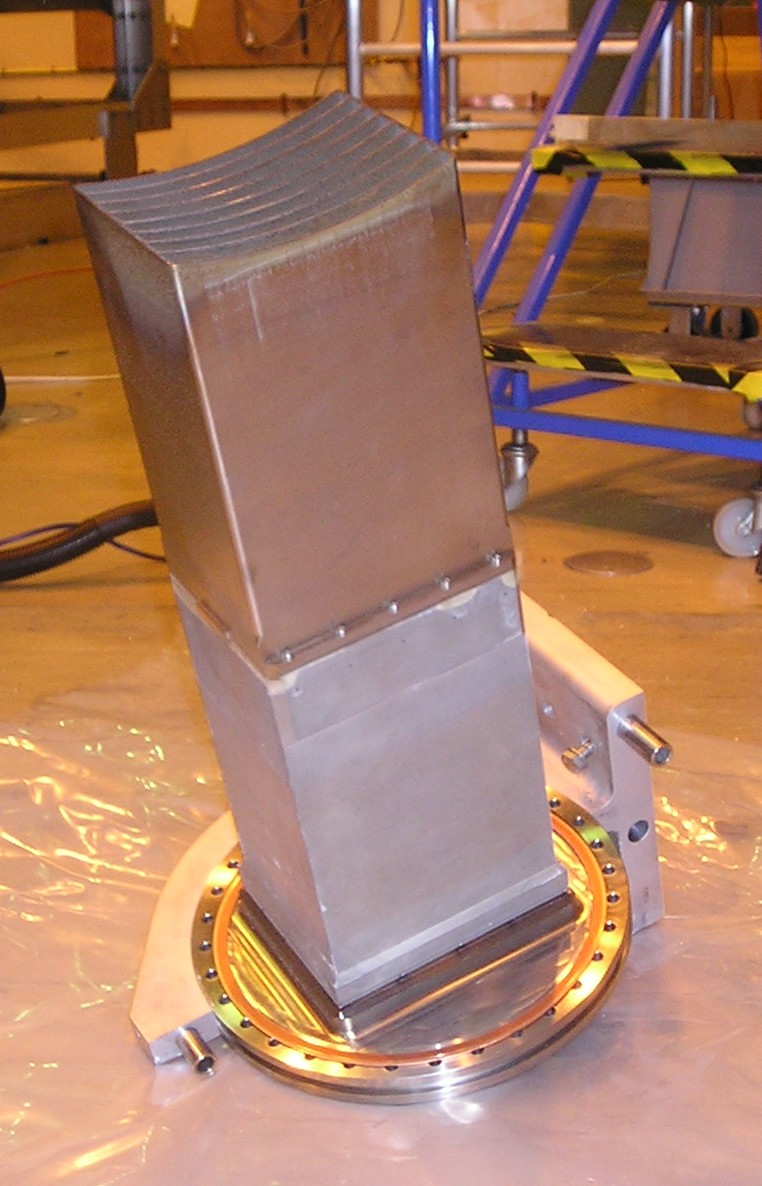
\includegraphics[width=0.4\linewidth]{Figures/LHCD/COMPASS_grill_out}
%	\caption{Picture of the grill mouth of the COMPASS-D LH launcher, made of 8 waveguides. Generator frequency was 1.3 GHz.}
%	\label{fig:compassgrillout}
%\end{figure}
%
%\begin{figure}
%	\centering
%	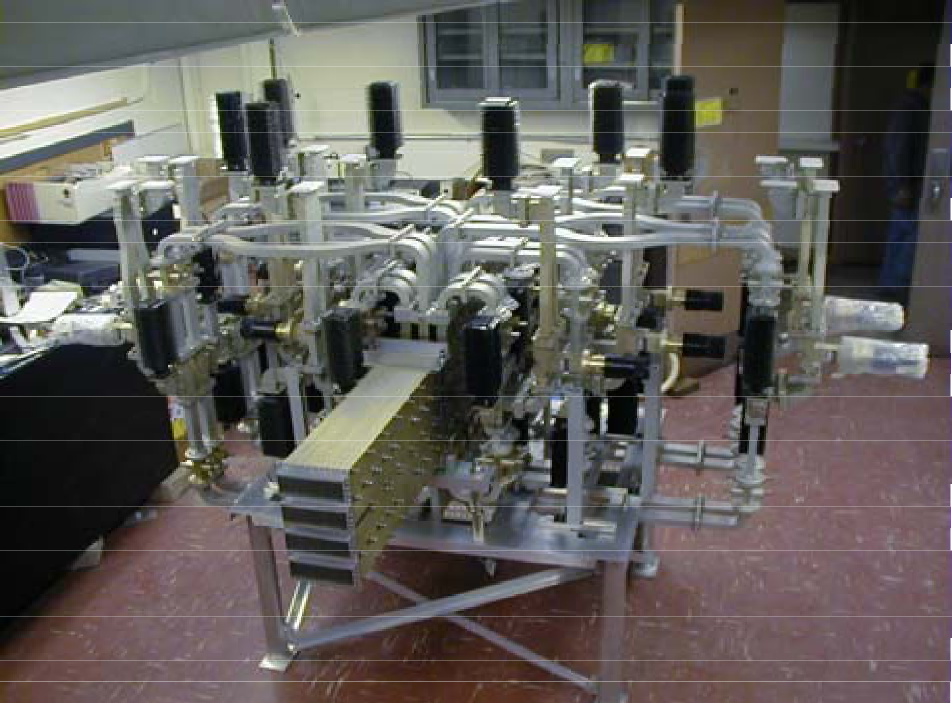
\includegraphics[width=0.7\linewidth]{Figures/LHCD/CMod_LH1}
%	\caption{The Alcator C-Mod LH1 launcher (88 waveguides, 4.6 GHz) and it associated transmission line (aka the”jungle gym”).}
%	\label{fig:cmodlh1}
%\end{figure}

\subsection{Multijunction Launchers}
In a large tokamak, a conventional LH grill made of independently fed waveguides would require hundred of waveguides, leading to a very complex power splitting design behind the antenna (cf.Figure \ref{fig:cmodlh1}). The use of \emph{multijunction} grill was suggested in 1984 to overcome this limitation \sidecite{Gormezano1985, Moreau1984}. In a multijunction grill, the main waveguide is divided into $N$ smaller (secondary waveguides) by thin metallic walls parallels to the wall of the main waveguide and perpendicular to the electric field: the \emph{E-plane N-junctions}. Built-in phase shifters made by reducing the waveguide height (in order to increase the guided wave phase velocity) are added in the structure in order to obtain the desired output phasing of the grill. Multijunction launcher makes it simpler to create and feed a large number or waveguides, at the contrary of classic grills launchers. However, a drawback is that the adjustment range of the power density spectrum is limited to a smaller range than for classic grills launchers.

A judicious choice of the phasing of the output waveguides leads to an important self-matching property of the multijunction (also known as \emph{recycling effect} or \emph{load resilience}). Indeed, for specific phase values, the reflected waves from the plasma which return back in the secondary waveguides can be reflected back to the plasma, thus leading to multiple reflections in the secondary waveguides. This recycling effect, which takes place between the plasma-antenna discontinuity and the E-plane bi-junctions, leads to an attenuation of the waves at each passage by the plasma, and ultimately to a decrease of the reflected power toward the RF sources. 

TODO: Illustration of the recycling effect (load resilience) inside a multijunction.


%\begin{figure}
%	\centering
%	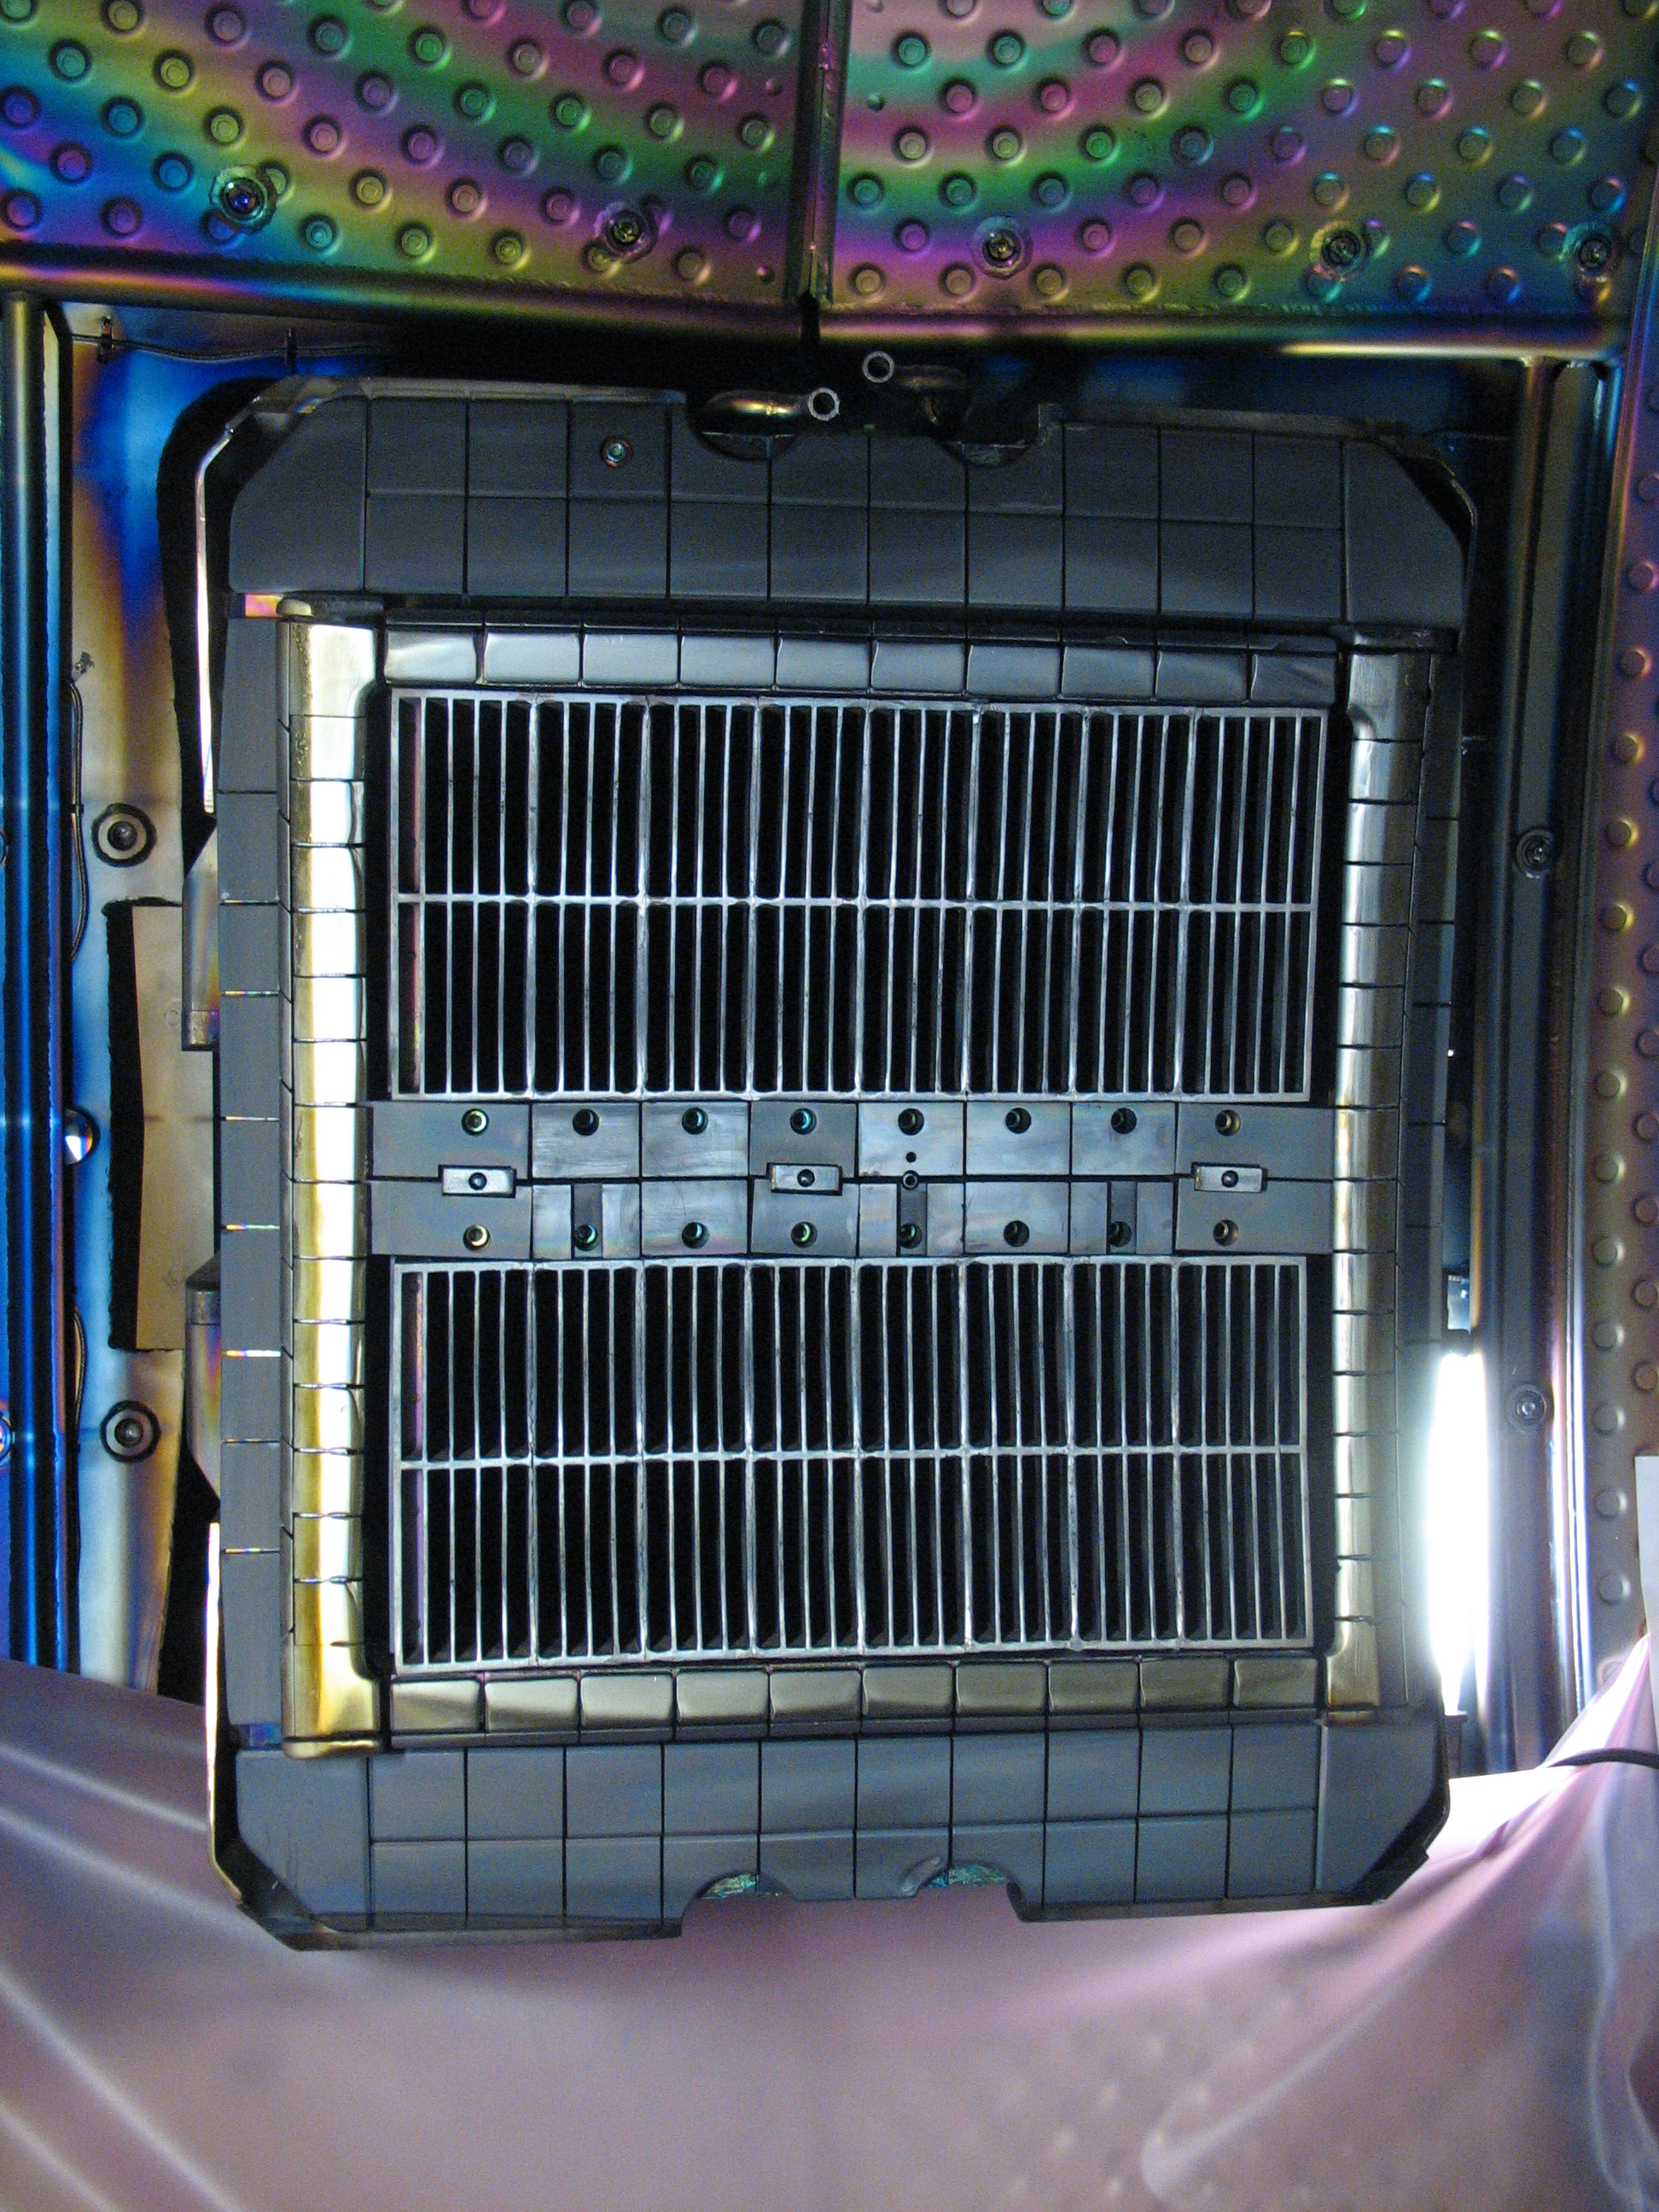
\includegraphics[width=0.3\linewidth]{Figures/LHCD/ToreSupra_C2}
%	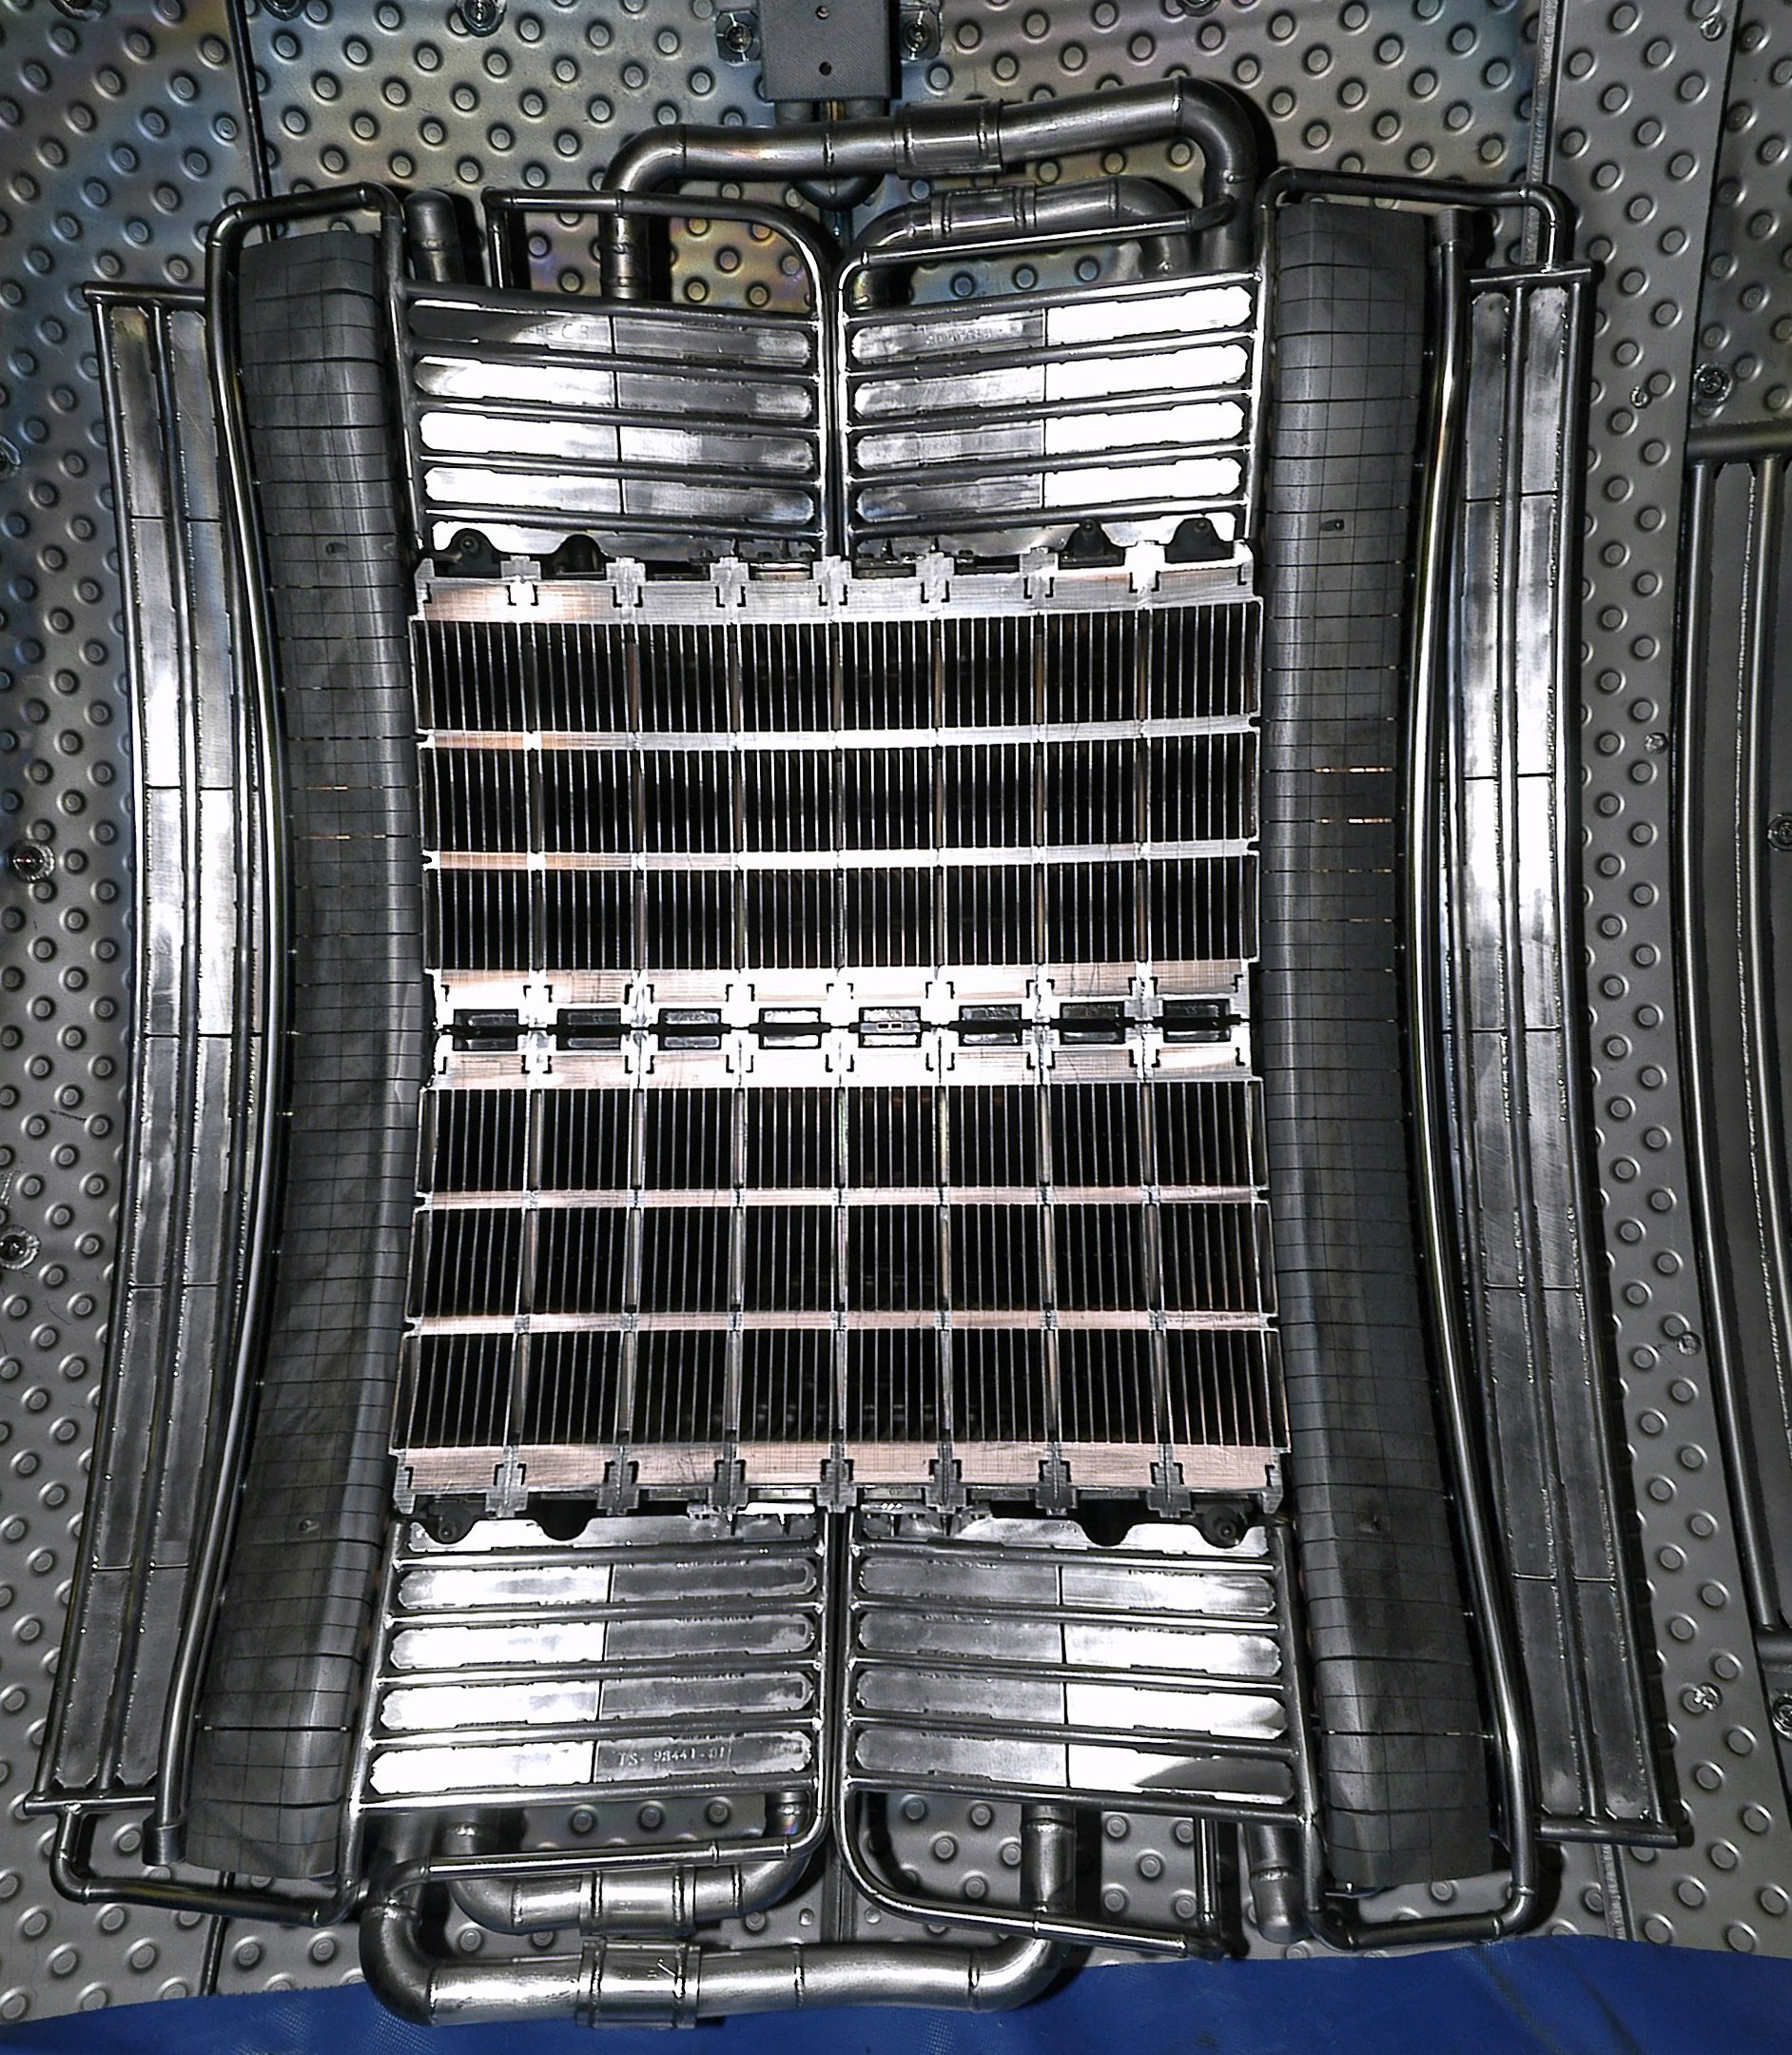
\includegraphics[width=0.4\linewidth]{Figures/LHCD/ToreSupra_C3}
%	\caption{Left:The Tore Supra Multijunction launchers as view from inside the vacuum vessel. The C2 launcher (128 waveguides, total dimensions 50 x 40 cm, 1989). Right: The C3 launcher (288 waveguides, total dimensions 60cm x 60cm, 1999). Frequency: 3.7GHz.}
%	\label{fig:toresupraC2C3}
%\end{figure}


\subsection{Passive-Active waveguide array launchers}
One of the main show-stopper to the use of LHCD to realize long and efficient pulses (outside the constraints of the tokamak magnetic coils heating) is the ability to couple high LH power to the plasma. Indeed, in order to achieve good coupling, the electron density in front of the LH launchers needs to be large enough, which means that the launcher needs to be located close enough to the plasma or to increase the local density by gas puffing means. 

The alternation of \emph{passive} waveguide (a waveguide closed by a short-circuit) and \emph{active} waveguide (a waveguide that is directly fed from the generator) has been initially proposed by Motley and Hooke \sidecite{Motley1980} in order to minimize the \emph{surface wave} excitation. Moreover, it was found that adding passive waveguide at each side of the array leads to decrease the reflected power in the last active guide \sidecite{Krapchev1978, Motley1980B}. The passive waveguides act as reflectors, radiating back a part of the power reflected by the plasma, and thus improving the coupling efficiency. Passive-Active grills were envisaged since the 1980' for fusion-reactor grade devices \sidecite{Ehst1982}. In these first conceptual designs, the passive waveguides were thought to be plugged or tuned individually in order for the outgoing power to have the requisite phase corresponding to an all-active grill system. 

Being close to the plasma leads to increase the heat fluxes into on the launcher front face. Thus, in order to improve the cooling of the launcher front face, it has been proposed in 1995 to insert one passive waveguide between each active waveguide, behind which a water pipe could efficiently water-cool the structure \sidecite{Bibet1995}. 

In order to insure a lower reflected power than a conventional grill, it has been proposed to associate this alternation of passive-active waveguide to  use a multijunction. This Passive-Active Multijunction (PAM) concept addresses two of the main criticisms made to LH launchers, i.e. the coupling efficiency and the heat loads resilience. 


\sidecite{kim2017, kim2019-1}

HFS KSTAR\sidecite{kim2019}


%\begin{figure}
%	\centering
%	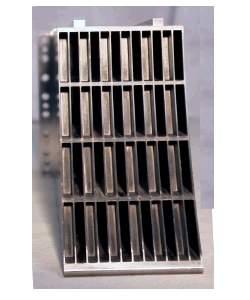
\includegraphics[width=0.4\linewidth]{Figures/LHCD/Pam_FTU}
%	\caption{PAM prototype tested on the FTU tokamak (24 active waveguides, 24 passive waveguides, 8 GHz, 2003) \sidecite{Mirizzi2003, Ridolfini2005}.}
%	\label{fig:pamftu}
%\end{figure}
%
%
%
%\begin{figure}
%	\centering
%	\includegraphics[width=0.6\linewidth]{Figures/LHCD/dsc_6078_dxo_2}
%	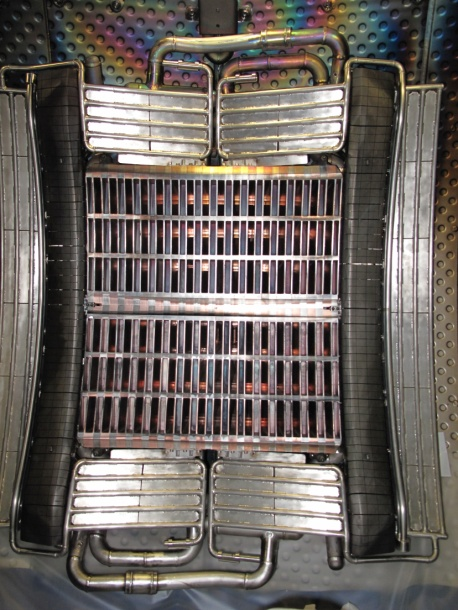
\includegraphics[width=0.3\linewidth]{Figures/LHCD/ToreSupra_C4}
%	\caption{The Tore Supra PAM (C4) launcher (96 active waveguides, 102 passive waveguides, approx. 7 tons, front face dimensions 60cm x 60cm, 3.7 GHz, 2009) \sidecite{Guilhem2009, Guilhem2011}.}
%	\label{fig:toresupraC4}
%\end{figure}


\subsection{Poloidal splitter launchers}
Motivated by the reduction of the RF losses and the increase of the reliability of a LH launcher, while keeping the flexibility in the parallel index $n_{\parallel}$ spectrum of the “grill” configuration (at the contrary of multijunction), the Alcator C-Mod team developed in 2008 a launcher (LH2) based on a four way splitter \sidecite{Koert2008a}. At the contrary of multijunction launcher, the four way splitter divides the power in the poloidal direction. Since the power splitting is done poloidally, the launched parallel power spectrum can be changed with the same flexibility as with conventional grill antennas. This design simplified the feeding structure of the antenna, thus reducing the RF losses due to multiple power splitters and flanges of previous grill configurations, while keeping a simple manufacturing assembly. The RF power is redistributed depending on the plasma load on each of the four rows of the splitter. If the load is the same for each row, the power is evenly split among rows. The RF optimization of the launcher has been made for a source frequency of 4.6 GHz and assuming a simplified plasma load (constant) in front of each row. A similar design has been made for the KSTAR tokamak, at 5 GHz \sidecite{Kim2012}. 


%\begin{figure}
%	\centering
%	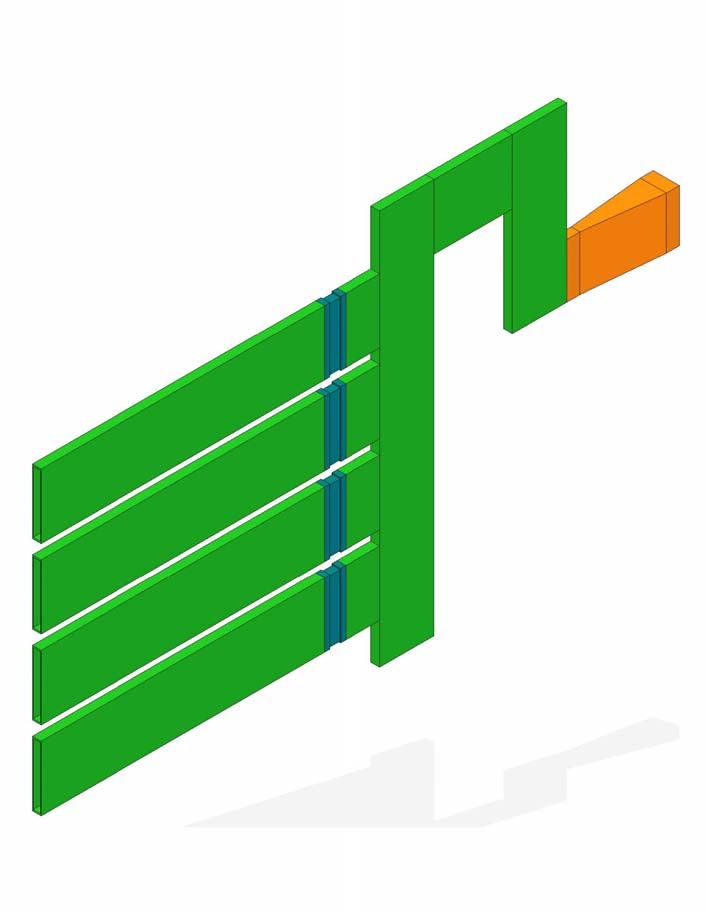
\includegraphics[width=0.4\linewidth]{Figures/LHCD/FourWaySplitter_1module}
%	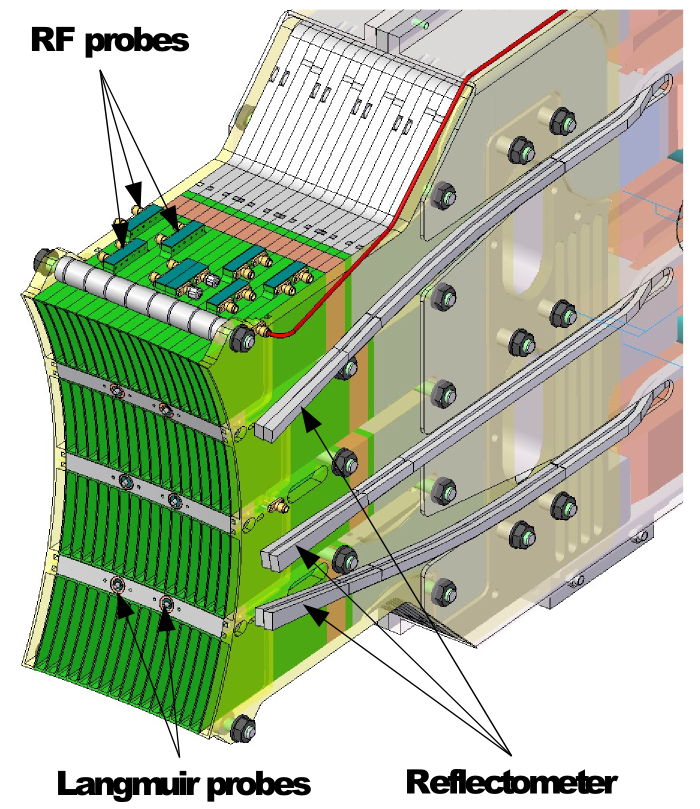
\includegraphics[width=0.4\linewidth]{Figures/LHCD/FourWaySplitter_CAD}
%	\caption{Left: CAD conceptual schematics of the four-way splitter of Alcator C-Mod \sidecite{Koert2008a}.Right: final assembly CAD model with 16 four-way splitters \sidecite{Meneghini2010b}.}
%	\label{fig:fourwaysplitter1module}
%\end{figure}
%
%
%\begin{figure}
%	\centering
%	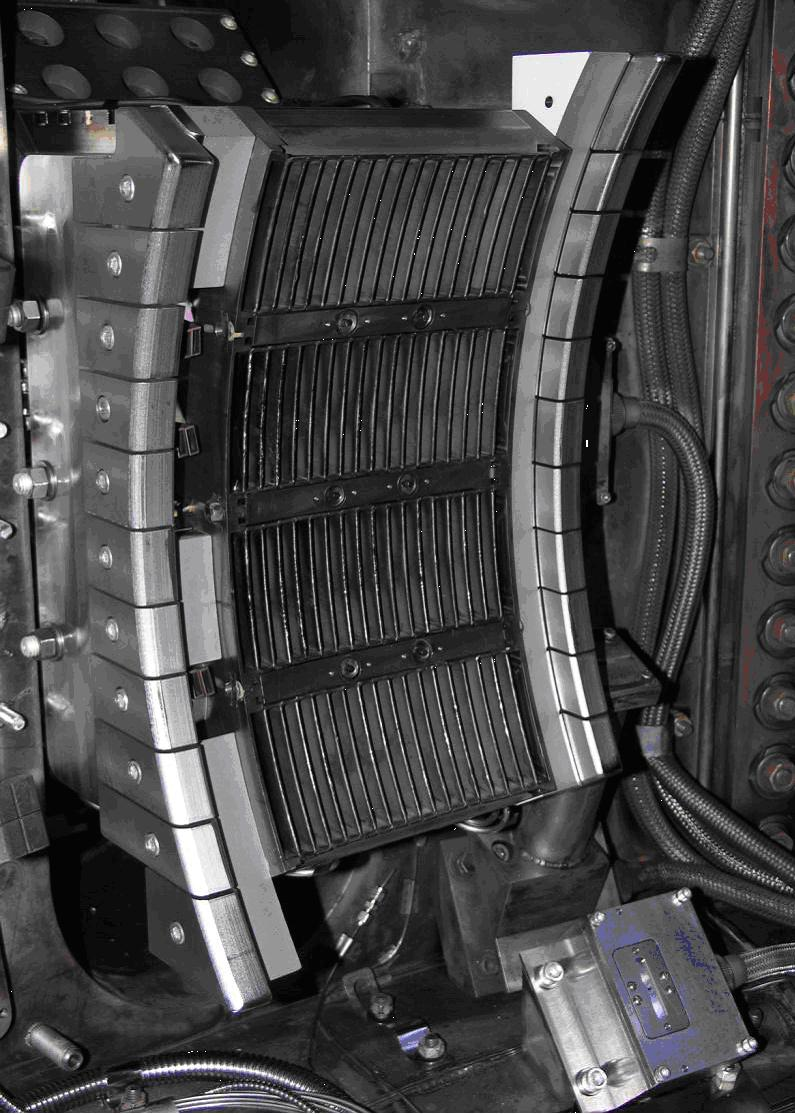
\includegraphics[width=0.4\linewidth]{Figures/LHCD/CMod_LH2}
%	\caption{Picture of the LH2 launcher inside the Alcator C-Mod vacuum vessel with its lateral protections in January 2012 \sidecite{Meneghini2010b}.}
%	\label{fig:cmodlh2}
%\end{figure}


\subsection{Wave propagation and absorption in the plasma}
In order for the RF power to reach the plasma core, the excited waves by a LHCD launcher must satisfy different criteria: 

\begin{itemize}
	\item  A \emph{cut-off condition}: the electron density in front of the launcher must be close or higher than the slow-wave electron \emph{cut-off density}. This density is given by:
	$$
	n_{c,\mathrm{cut-off}} = \varepsilon_0 m_e \frac{\omega^2}{e^2}
	$$
	and thus increases as the square of the source frequency. 
	\item A propagation condition: in order for the LH waves to propagate into the magnetized plasma, excited waves must have an absolute value of the parallel index greater than one, i.e. $|n_{\parallel}|>1$ 
	\item An accessibility condition: in order for the slow waves which access to the core plasma not to be mode-converted into fast waves, a minimum value of $n_{\parallel}$ for a given plasma density and magnetic field is requested :
	$$
	|n_{\parallel} |>| n_{\parallel \mathrm{access}} | 
	\approx 
	\sqrt{1 
		- \frac{\omega_{pi}^2}{\omega^2} 
		+ \frac{\omega_{pe}^2}{\omega_{ce}^2}}
	+ \frac{\omega_{pe} }{| \omega_{ce} |}
	$$ 
	When the accessibility condition is satisfied, the slow and the fast branch of the dispersion relation are separated and the LH waves can reach the core plasma.
	Inversely, for a given $n_{\parallel}$, the previous condition leads to an upper limit for the density, above which the wave can’t propagate.
\end{itemize}

%\begin{figure}
%	\centering
%	\includegraphics[width=0.9\linewidth]{Figures/LHCD/C3_powerflow}
%	\caption{Illustration of the power density radiated by a LH launcher (seen into a horizontal plane cut) into a plasma of increasing electron density. The plasma current direction is indicated. Since the launcher is designed to launch a non-symmetrical power spectrum, the power flows toward a preferred direction (opposite to the plasma current).}
%	\label{fig:c3powerflow}
%\end{figure}



The RF power is coupled by the launcher to the plasma, which means that the electromagnetic waves in the launcher’s waveguides are converted to (mainly) slow waves in the plasma. In the LH range of frequencies (~2 to 8 GHz), the wavelength of the RF waves in the plasma is well below the typical beam size, which itself is smaller than the equilibrium non-uniformity scale. It this situation, the evolution of the waves in the plasma can be described by the \emph{ray-tracing} formalism. Since the evolution of the electron population can be described with Fokker-Planck calculation, the combination of the both tools is standard for modelling LHCD experiments\sidecite{Bonoli1982, Peysson2012}.

As said before, the LHCD launcher is a phased array of waveguide which excites a slow plasma wave. The following calculations taken from current drive theory illustrate the basic requirements of the LHCD launcher in order to optimize the current drive efficiency. 

In the plasma, the incremental current $\Delta j$ carried by an electron of electrical charge $q=-e$ and accelerated from a parallel velocity $v_\parallel$ to $v_\parallel + \Delta v_\parallel$ is:
$$\Delta j = q \Delta v_{\parallel}$$

The incremental increase of kinetic energy is:
$$\Delta E = m v_{\parallel} \Delta v_{\parallel}$$

Eliminating $\Delta v_{\parallel}$ leads to an incremental current: 
$$\Delta j = \Delta E \; q/(m v_{\parallel})$$ 

Let $\nu_\mathrm{coll}$ be the Coulomb collisional frequency. At first order \footnote{Rigourously, the mathematical tool for a complete description of multiple scattering processes in the velocity-space is the Boltzman equation. The collision term modelling the multiple particles Coulomb collisions in this equation can be modelled by a collision term of the Fokker-Planck type.} the incremental energy input $\Delta E$ persists for a time $1/\nu_\mathrm{coll}$. The associated (steady-state) RF input power $\Delta P$ required is thus: 
$$\Delta P = \nu_\mathrm{coll} \Delta E$$ 

From the two previous equations, the ratio of the incremental current to the RF input power is:
$$\Delta j/ \Delta P = q / (m \nu_\mathrm{coll} v_{\parallel})$$

This suggests that more current can be driven with low parallel velocity electrons. However, fast electrons collide less often than slower, as the Coulomb collision cross section falls off with increasing relative velocity as $\nu_\mathrm{coll} \propto n_e/v_{\parallel}^3$ (for parallel velocity larger than the thermal velocity). It follows that the previous ratio is proportional to: 

$$\Delta j/ \Delta P \propto (v_{\parallel}^2 q) / (m n_e)$$

this means that high current drive efficiency can be reached from fast electrons. Thus, it is actually more effective to push fast electrons than slower. Even if it may be energetically more expensive to accelerate fast electrons, this energy deposition need occurs less often because current last longer when carried by relatively less collisional electrons \sidecite{Fisch1987}. 

For the purpose of current drive with LH waves, the Landau damping is the dominant absorption mechanism. Landau damping is a collision-less damping process in which particles exchange energy with waves travelling with the nearly same phase velocity parallel to the magnetic field, that is, for particle parallel velocity $v_{\parallel}$ satisfying resonant condition:

$$\omega – k_{\parallel} v_{\parallel} = 0 $$ 

where $k_{\parallel}=k_0 n_{\parallel}$ is the parallel wavenumber of the wave, $n_{\parallel}$ the parallel index of refraction and $k_0= \omega/c$ the wavenumber in vacuum. From the previous relation one deduces that the LHCD launcher must excite waves satisfying the resonant condition $v_{\parallel}=c/n_{\parallel}$. As for the slow wave to be able to penetrate into the plasma the parallel index must be greater than one and also greater to $|n_{\parallel \mathrm{access}}|$, typical LHCD launchers in current tokamaks excite a main parallel index between $n_{\parallel 0}$=1.5 to 3.0. 

However, in many past and present LHCD experiments, the resonant velocity $v_{\parallel 0}=c/n_{\parallel 0}$ corresponds to supra thermal region where the number of electrons should be in principle too small for any significant wave damping to take place and to account for the observed current drive. Indeed, strong wave damping on a Maxwellian distribution with temperature $T$ requires the wave damping to be no larger than four times the thermal velocity $v_T=\sqrt{k T/m}$. This paradox is commonly referred to as the \emph{spectral gap} problem and is an active area of research. Various explanations are proposed to explain this spectral gap, among these the toroidal effects on the wave propagation that can cause sufficient up-shift (increase of the parallel wavenumber) in the parallel refraction index $n_{\parallel}$ to “fill” the spectral gap, non-linear interactions such as \textit{parametric decay instabilities} (PDI), diffraction effects or power density spectrum fluctuations. 


\subsection{Resonance Cone}
Bellan and Porkolab PRL 34, 124, 1975.


\subsection{Overview of parameters achieved and example of some systems}
\subsubsection{LH Launchers main figures of merit}

There are three important figures of merit to measure the efficiency and the performances of a LH launcher: 
\begin{enumerate}
	\item The first one is the k-space radiated power spectrum, generally characterized by its \emph{parallel power spectrum} $p(n_{\parallel})$ . This quantity represents the amount of power for each parallel index excited by the launcher. The relation between this power spectrum and the array excitation is related to the Fourier transform of the electromagnetic field at the plasma-antenna interface. 
	
	\item  The second one is the ratio of the reflected power (at the mouth or at the end of the launcher) to the input power, named the \emph{reflection coefficient} (sometime expressed in percent). 
	$$RC = \frac{P_r}{P_i}$$
	\item The third one is the \emph{directivity} of the launcher, which is the fraction of the power spectrum over its total power content. It can be viewed as the fraction of the power that goes toward one toroidal direction over the total coupled power. One can define the directivity as follow\footnote{Other definitions exist, essentially in order to ad a physical content to the directivity, in relation with the current drive efficiency evolution in the plasma. See for instance \sidecite{Litaudon1990a}.}
	$$
	D
	= 
	\frac{
		\int_{n_{\parallel} >0} p(n_{\parallel}) dn_{\parallel} 
	}{
		\int_{n_{\parallel}} p(n_{\parallel}) dn_{\parallel} } 
	$$
\end{enumerate}

Theoretically, if the $n_{\parallel}$ spectrum of an antenna is known, one can evaluate the reflection coefficient. However, since the wave field at the launcher aperture (and thus the launcher spectrum) depends on the plasma itself, numerical codes are required to make a self-consistent numerical evaluation of the coupling. Such codes are coupling codes.

\subsection{LH systems and launchers performances}
Mainly because of its relative simplicity, most of the LH launchers have been based on a "grill" configuration, as for example in the 1980' \sidecite{porkolab1984a, gormezano1986a, Stevens1988}.

Typical grill launchers have a high reflection coefficient (of the order of 20 to 40\%) but directivity higher than 80\%. Since all the waveguides can be feed by independent RF sources, and thus independently phased, such launchers have a wide flexibility in terms of operational space (excited spectrum) which is of great interest for physics studies. However, since each waveguide is independently power fed, the complexity of the launcher grows enormously with the number of output waveguides, leading to cumbersome transmission systems for multi-megawatt power levels (Table \ref{tab:grillperformances}). 


Multijunction launchers at the contrary have led to hundred of waveguides launchers (see Table \ref{tab:multijunctionperformances}). The complexity of the multijunction design and manufacturing is balanced by the a simpler transmission line system behind the launcher. Because of the self-matching property, the typical reflection coefficient of multijunction launchers is generally less than 10\%. However, the multiple back and forth of the waves leads to an increase of the peak electric field in secondary waveguides. Moreover, since the phase shift is created by the built-in phase shifter inside the launcher, the flexibility of phase configuration is reduced in comparison to classic grill launchers. 


The PAM concept tested in FTU and in the Tore Supra tokamak showed that reflected power lower than 5\% (i.e. high coupling efficiency) and continuous operations could be combined (cf. Figure \ref{fig:ts45472c4ir}) during long pulse operations. 



\subsection{ITER System}

Although not part of the ITER initially planned procurement phase, a conceptual design of a 20~MW/CW 5~GHz LHCD system has been proposed for the second mission of ITER, i.e. Q=5 steady state target \sidecite{hoang2009}. In ITER, the parallel index of the launched waves $n_{\parallel 0}$ ~ 2.0 has been selected as a trade-off between the current drive efficiency, the wave accessibility and the location of power deposition, all of which depend upon the plasma conditions. Depending of the plasma scenarios (steady-state, hybrid, ramp-up, etc.), the additional current driven by LHCD would range between 0.42 MA (steady-state) up to more than 3.0 MA (ramp-up) \sidecite{decker2011}. In any case, these values confirm that for steady state scenarios, a substantial bootstrap current is required \sidecite{jacquinot1999}. The average current drive efficiency, which is the figure of merit of the LHCD, has been calculated to be $\eta \equiv 0.2 \times 10^{20} A m^{-2} W^{-1}$, similar to the ones measured in present days tokamaks \sidecite{jacquinot1999}. This value can be compared to other additional current drive scheme, such as NBI or ECCD. 

In addition, LHCD-assisted start-up could reduce the flux consumption during current ramp-up, resulting in a longer flat top or burn time. An early application of 20 MW LHCD during the plasma current ramp-up phase of the ITER reference scenario 2 is effective to reduce the flux consumption. An expected saved flux of 43Wb is equivalent to about 500 s of additional burn duration \sidecite{hoang2009}.

